\documentclass[11pt,a4paper]{article}

\usepackage[margin=1in]{geometry}
\usepackage[T1]{fontenc}
\usepackage[utf8]{inputenc}
\usepackage{lmodern}
\usepackage{microtype}
\usepackage{graphicx}
\usepackage{booktabs}
\usepackage{tabularx}
\usepackage{array}
\usepackage{multirow}
\usepackage{amsmath}
\usepackage{amssymb}
\usepackage{siunitx}
\usepackage{xcolor}
\usepackage{enumitem}
\usepackage{caption}
\usepackage{subcaption}
\usepackage{float}
\usepackage{hyperref}
\usepackage{cleveref}
\usepackage[numbers,sort&compress]{natbib}

\definecolor{navy}{HTML}{16324F}
\definecolor{teal}{HTML}{168AAD}
\definecolor{steel}{HTML}{557A95}
\definecolor{lightgray}{HTML}{F1F4F6}
\definecolor{warning}{HTML}{9B4D2A}

\hypersetup{
    colorlinks=true,
    linkcolor=navy,
    citecolor=teal,
    urlcolor=steel,
    pdftitle={BanglaSlumNet Project Report},
    pdfauthor={BanglaSlumNet Research Team}
}

\newcolumntype{Y}{>{\raggedright\arraybackslash}X}
\setlist[itemize]{leftmargin=*,nosep}
\setlist[enumerate]{leftmargin=*}
\captionsetup{font=small,labelfont=bf}

\newcommand{\project}{BanglaSlumNet}
\newcommand{\placeholderfigure}[3]{%
    \begin{figure}[H]
        \centering
        \IfFileExists{#1}{%
            \includegraphics[width=#2\linewidth]{#1}
        }{%
            \fcolorbox{steel}{lightgray}{%
                \begin{minipage}[c][0.24\textheight][c]{0.88\linewidth}
                    \centering
                    \textbf{Designer figure placeholder}\\[0.6em]
                    Expected file: \texttt{\detokenize{#1}}\\[0.6em]
                    See \texttt{diagram\_instructions.md}.
                \end{minipage}
            }
        }
        \caption{#3}
    \end{figure}
}

\title{\textbf{\project: Language-Grounded Socioeconomic Fusion\\
for Dense-Megacity Informal-Settlement Detection}}
\author{
Namare Shakib Angkon \and
Syed Zayan Anwar \and
Md. Abdullah Al Nafiz \and
Golam Bari Fardeen \and
Md. Masum Mizi
}
\date{Project report, June 2026}

\begin{document}

\maketitle

\begin{abstract}
Informal-settlement mapping from satellite imagery is difficult in dense megacities because visual density is not equivalent to informality. In Dhaka, tightly packed formal neighborhoods can resemble informal settlements in medium-resolution optical imagery, causing optical-only models to learn shortcuts based on roof density and urban texture. This report presents \project, an end-to-end research pipeline that combines Sentinel-2 imagery, language-grounded features from the LocateAnything vision-language model, scene-appearance normalization, and socioeconomic context. The work includes a multi-region Dhaka benchmark, a weak-supervision strategy based on known region type and built-up masks, cache-aware Colab orchestration, cross-attention fusion, controlled ablations, and extensive preflight and collapse diagnostics. During experimentation, we identified failures in the original weak-label rule and in early metric interpretation: apparent performance was partly caused by trivial all-positive or all-negative predictions. We corrected the data and evaluation pipeline, but the current evidence indicates that region-level weak supervision and coarse imagery are insufficient for strong pixel-level claims. The main contribution at this stage is therefore a reproducible, compute-aware experimental foundation and a clear roadmap toward reliable evaluation through manual annotation, improved socioeconomic layers, high-resolution grounding, and a potentially more appropriate tile-level formulation.
\end{abstract}

\section{Introduction}

Accurate maps of informal settlements support urban planning, public-health interventions, infrastructure allocation, climate adaptation, and disaster response. Yet the spatial extent of such settlements is frequently absent from official data or changes faster than conventional surveys can document. Earth observation offers repeated, city-scale coverage and has therefore become an important complement to field mapping \citep{kuffer2016slums,mahabir2018critical}.

The problem is not merely to detect dense built-up areas. Informality is a social, infrastructural, and legal condition that only partially manifests in overhead imagery. Dhaka makes this distinction especially difficult: informal settlements such as Korail coexist with dense formal districts and historic masonry cores whose visible texture may be similarly compact and irregular. A model trained only on optical patterns can consequently learn a shortcut in which ``dense'' becomes synonymous with ``slum.''

Prior work has demonstrated that informal settlements can be mapped with handcrafted features, object-based analysis, classical machine learning, convolutional neural networks, and freely available Sentinel-2 imagery \citep{kuffer2016slums,mboga2017detection,gramhansen2019mapping,matarira2022gee}. However, these approaches remain constrained by geographic transfer, label scarcity, image resolution, and uncertainty \citep{fisher2022uncertainty}. Work on poverty estimation also shows that non-visual signals such as nighttime illumination can complement daytime imagery \citep{jean2016poverty}.

\project\ explores whether this ambiguity can be reduced by combining three sources of evidence:

\begin{enumerate}
    \item optical structure from Sentinel-2 imagery;
    \item language-grounded visual features that encode the conceptual contrast between informal and dense-formal settlement; and
    \item socioeconomic context, including nighttime lights, population, accessibility, and built-up extent.
\end{enumerate}

The project is organized around the following research questions:

\begin{enumerate}
    \item How can informal settlements be distinguished from visually similar dense formal neighborhoods in Dhaka?
    \item Does language grounding provide information beyond neutral visual features?
    \item Can socioeconomic layers reduce false-positive predictions in dense formal control regions?
\end{enumerate}

The present report documents the complete development path, including failed assumptions, engineering corrections, current diagnostic results, and the changes required before strong scientific claims are made.

\section{Literature Review}

\subsection{Remote Sensing of Informal Settlements}

The remote-sensing literature has long emphasized that slum morphology is heterogeneous across cities. Kuffer, Pfeffer, and Sliuzas reviewed fifteen years of slum mapping and identified recurring features such as high building density, irregular layout, small roof size, and limited road access, while also stressing the absence of a universal image signature \citep{kuffer2016slums}. Mahabir et al.\ similarly reviewed high- and very-high-resolution methods and highlighted geographic concentration, inconsistent definitions, and transferability as persistent challenges \citep{mahabir2018critical}.

Object-based and texture-driven methods offered interpretable ways to characterize informal morphology, but required city-specific feature engineering. The move toward learned representations enabled convolutional models to identify spatial patterns directly. Mboga et al.\ used CNN-derived features for informal-settlement detection in very-high-resolution imagery and showed the value of contextual structure over purely pixel-based classification \citep{mboga2017detection}. Gram-Hansen et al.\ compared low-resolution spectral classification with a high-resolution semantic-segmentation approach and released benchmark data, demonstrating both the scalability of Sentinel-2 and the importance of fine spatial context \citep{gramhansen2019mapping}.

Recent work has explored cloud platforms and uncertainty-aware deep learning. Matarira et al.\ used Google Earth Engine with Sentinel-2 spectral and textural variables to map heterogeneous informal settlements \citep{matarira2022gee}. Fisher et al.\ combined U-Net segmentation, uncertainty estimation, and interpretability, emphasizing that model confidence must be examined alongside headline accuracy \citep{fisher2022uncertainty}. These findings directly motivated our decision to add explicit collapse diagnostics rather than rely only on intersection-over-union.

\subsection{Segmentation Architectures}

U-Net established the encoder--decoder pattern with skip connections for precise pixel localization under limited annotation \citep{ronneberger2015unet}. SegFormer later combined a hierarchical transformer encoder with a lightweight decoder, providing an efficient optical baseline for semantic segmentation \citep{xie2021segformer}. \project\ uses a lightweight U-Net-style decoder for cached VLM features and retains a SegFormer-like optical baseline for controlled comparison.

\subsection{Vision--Language Grounding}

Vision--language models connect free-form text with image content. LocateAnything is a recent generative visual-grounding framework designed to localize prompted concepts through parallel box decoding \citep{wang2026locateanything}. Its intended domains extend beyond remote sensing, but its prompt-conditioned localization provides a useful experimental mechanism: the same image can be queried with neutral, informal-settlement, and dense-formal descriptions. In \project, the large VLM is frozen and used only to generate cached grounding maps. This avoids costly end-to-end fine-tuning while preserving prompt dependence.

\subsection{Socioeconomic and Geospatial Context}

The use of satellite proxies for socioeconomic inference is well established. Jean et al.\ combined nighttime illumination and daytime imagery to estimate poverty, illustrating the complementary value of non-visual socioeconomic evidence \citep{jean2016poverty}. Our socioeconomic tensor draws from VIIRS nighttime light, WorldPop and GHS population products, road/accessibility information, and GHSL built-up extent.

Sentinel-2 provides multispectral observations suitable for repeated land monitoring \citep{drusch2012sentinel2}. Google Earth Engine supports scalable access and processing of these archives \citep{gorelick2017gee}. Dynamic World provides near-real-time land-cover probabilities at Sentinel-2 scale and is used here as one component of the built-up mask \citep{brown2022dynamicworld}. GHSL and WorldPop provide complementary settlement and population context, though their coarser native scales and model assumptions must be acknowledged.

\subsection{Attention and Appearance Normalization}

The fusion module is based on attention, in which visual tokens query projected socioeconomic tokens. Attention mechanisms were popularized by the Transformer architecture \citep{vaswani2017attention}. The Stage-1 appearance-normalization design uses an AdaIN-inspired separation of scene content and appearance statistics \citep{huang2017adain}. Our SAS-Net implementation is project-specific rather than a direct reproduction of an external named architecture.

\section{Dataset}

\subsection{Study Area and Collection Strategy}

We created a Dhaka-focused weak-supervision benchmark because existing public informal-settlement datasets do not represent the specific dense-formal confusion targeted by this study. The benchmark contains eight regions treated as informal and four deliberately difficult formal-dense controls. The controls are not random background: Old Dhaka, Gulshan--Baridhara, Dhanmondi, and Uttara were selected because their density or urban texture can resemble informal morphology.

\begin{table}[H]
\centering
\caption{Region groups used in the benchmark.}
\begin{tabularx}{\linewidth}{YY}
\toprule
\textbf{Informal target regions} & \textbf{Formal-dense control regions}\\
\midrule
Korail; Bhashantek; Karail extension; Kamrangirchar; Kallyanpur; Hazaribagh; Tongi; Mirpur Beribadh
&
Old Dhaka; Gulshan--Baridhara; Dhanmondi; Uttara\\
\bottomrule
\end{tabularx}
\end{table}

Sentinel-2 Level-2A dry-season composites were exported for multiple years using Google Earth Engine. The principal optical channels were blue, green, red, and near-infrared. Wet-season exports were attempted but frequently contained insufficient valid observations because of monsoon cloud cover. The implemented pipeline therefore uses the available dry-season composites and reports seasonal coverage as a limitation.

Regional images were tiled into \(128\times128\) pixel samples, corresponding to approximately \(1.28\) km on each side at the nominal Sentinel-2 resolution. Overlapping strides were used for training coverage. The resulting manifest contained 720 tile records, stratified by region into training, validation, and test subsets.

\subsection{Supporting Data Sources}

\begin{table}[H]
\centering
\caption{Geospatial layers used or planned in the current pipeline.}
\begin{tabularx}{\linewidth}{p{0.22\linewidth}Yp{0.19\linewidth}}
\toprule
\textbf{Layer} & \textbf{Role} & \textbf{Current status}\\
\midrule
Sentinel-2 L2A & Optical imagery and spatial reference grid & Operational\\
Dynamic World & Built-class evidence for weak labeling & Operational\\
GHSL built-up & Built-surface evidence and socioeconomic context & Operational\\
WorldPop / GHS-POP & Population-density context & Operational\\
VIIRS nighttime light & Electricity/economic-activity proxy & Operational\\
Road accessibility & Connectivity proxy & Placeholder proxy\\
Poverty layer & Deprivation context & Zero placeholder\\
\bottomrule
\end{tabularx}
\end{table}

\subsection{Annotation and Weak-Supervision Process}

The original annotation rule attempted to divide built pixels into slum and formal classes using a city-level VIIRS dark/bright threshold. In the real exports, that rule collapsed to an all-formal label set. Because the failure would make every later experiment meaningless, a CPU-side verification gate was added and the labeling rule was redesigned.

The current rule is:

\begin{equation}
y(p)=
\begin{cases}
1, & p\in B \text{ and region}(p)\text{ is informal},\\
2, & p\in B \text{ and region}(p)\text{ is formal control},\\
0, & p\notin B,
\end{cases}
\end{equation}

where \(B\) is the union of GHSL built-up evidence and the Dynamic World built class. Class \(0\) is ignored, class \(1\) denotes slum, and class \(2\) denotes formal-dense built-up. The high-confidence mask is currently the built portion of each known region.

The verification gate confirmed that both classes were present and that high-confidence pixels were non-empty. This solved the zero-slum implementation failure, but it did not convert the labels into true pixel-level ground truth. The labels encode region identity on built pixels and may therefore reward region-specific shortcuts.

\subsection{Alignment and Augmentation}

All supporting rasters are reprojected onto each Sentinel-2 tile grid using nearest-neighbor resampling for labels and bilinear resampling for continuous socioeconomic layers. Shape and geotransform assertions fail loudly if alignment is inconsistent. This design was adopted because silent label misalignment would be more damaging than a visible runtime error.

Training augmentation applies the same random horizontal flip, vertical flip, and \(90^\circ\) rotation to RGB imagery, labels, high-confidence masks, and socioeconomic tensors. Augmentation increases orientation diversity but cannot compensate for coarse or systematically biased labels.

\subsection{Representative Samples}

\begin{figure}[H]
    \centering
    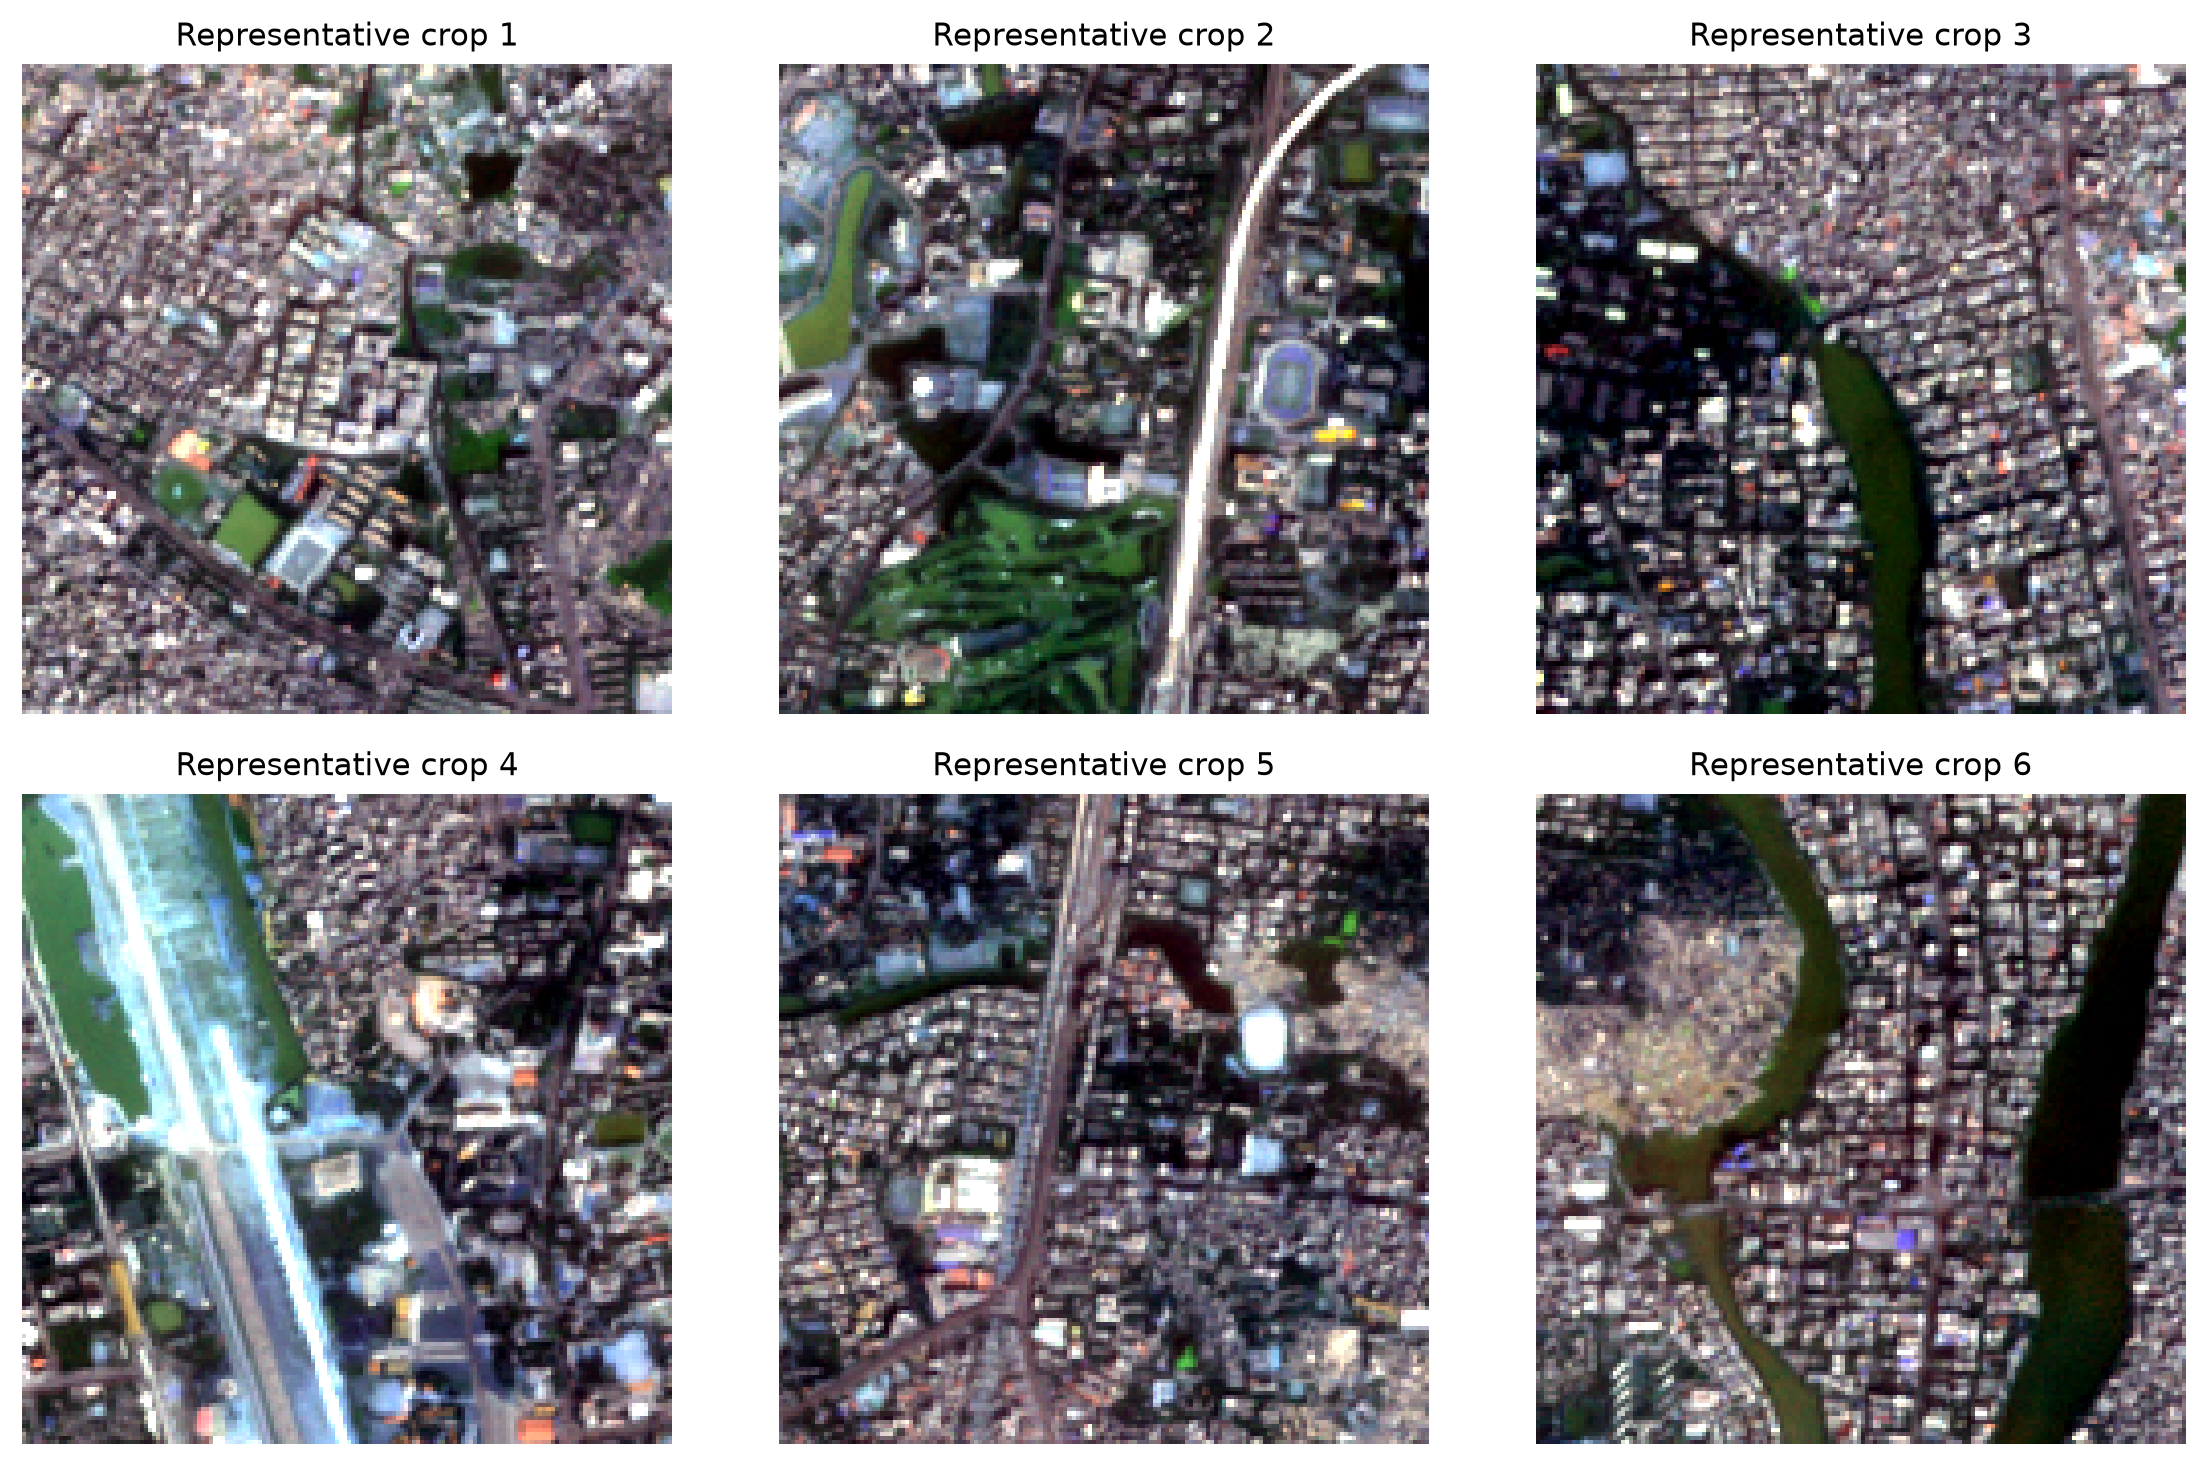
\includegraphics[width=0.95\linewidth]{figures/dataset_samples.png}
    \caption{Six representative crops rendered from the locally available Dhaka Sentinel-2 composite. These samples illustrate the visual scale and heterogeneity of the imagery, but they should not be interpreted as six independently verified region labels.}
    \label{fig:samples}
\end{figure}

\begin{figure}[H]
    \centering
    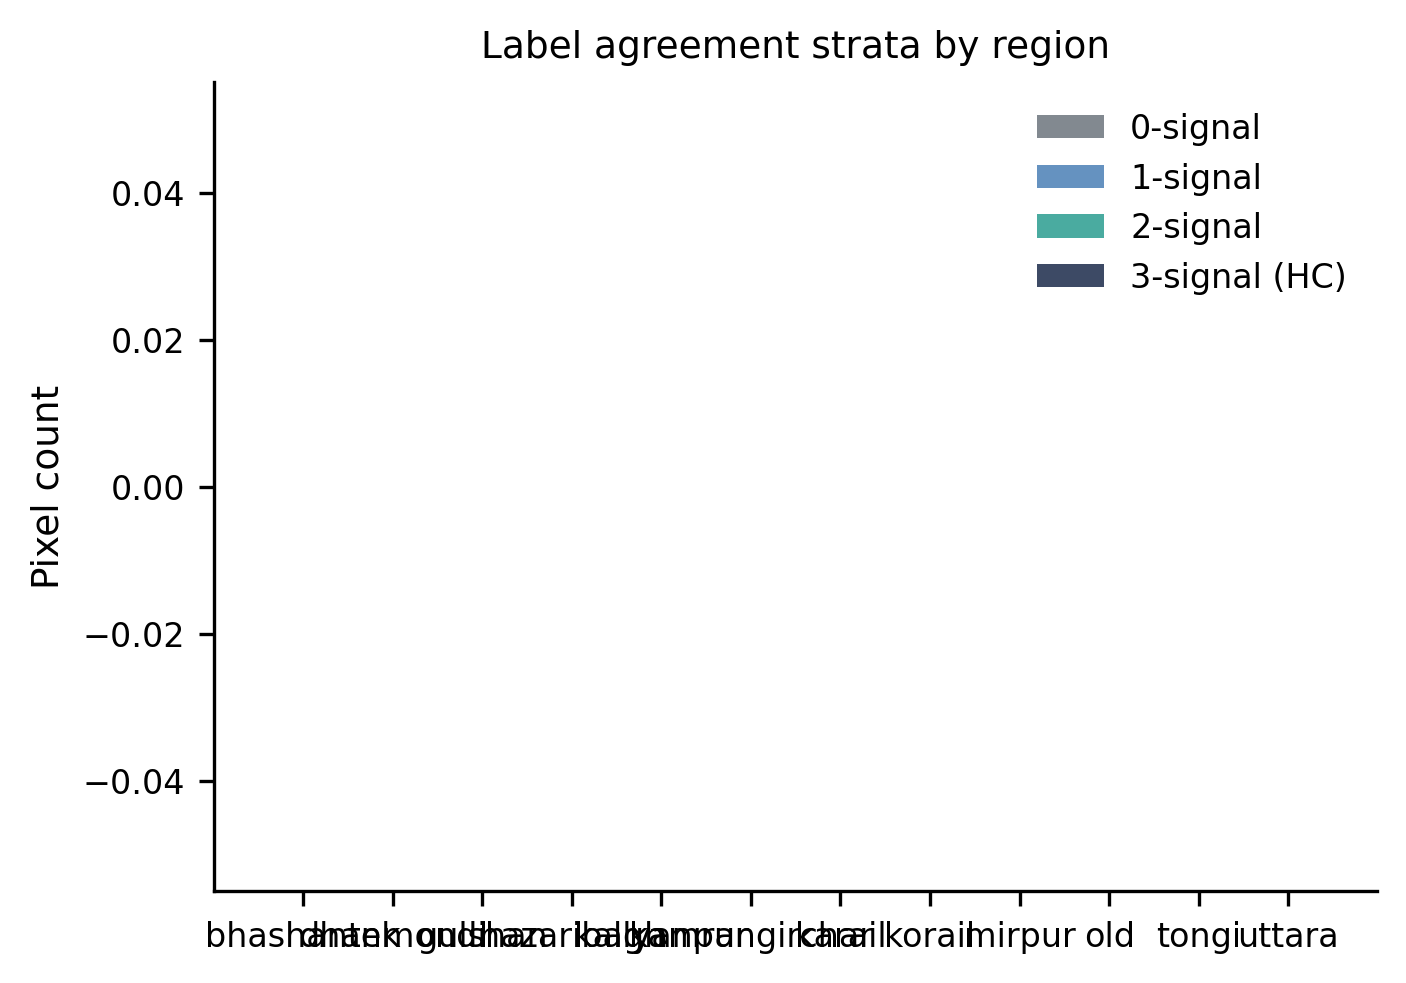
\includegraphics[width=0.72\linewidth]{figures/confidence_strata.png}
    \caption{Confidence-strata visualization generated by the project pipeline. The figure is retained as a data-audit artifact rather than evidence of final predictive performance.}
\end{figure}

\section{Methodology and Architecture}

\subsection{System Overview}

\placeholderfigure{figures/system_architecture.pdf}{0.98}{Proposed \project\ architecture. Sentinel-2 imagery is normalized by SAS-Net; prompt-conditioned LocateAnything features are fused with socioeconomic layers through cross-attention; a lightweight decoder produces a slum-probability mask.}

The system has two main stages. Stage 1 reduces appearance variability, while Stage 2 combines cached visual-language features with socioeconomic context. Only the projection, fusion, and decoder components are trained during the main experiment; the LocateAnything backbone remains frozen.

\subsection{Stage 1: Scene--Appearance Separation}

SAS-Net encodes scene structure and appearance statistics separately. An AdaIN-inspired renderer reconstructs the image and supports appearance swapping between observations. The training objective combines reconstruction, scene consistency, and appearance-swap losses:

\begin{equation}
\mathcal{L}_{\text{SAS}} =
\lambda_{\text{rec}}\mathcal{L}_{1}(I,\hat{I})+
\lambda_{\text{cons}}\|E_s(I_1)-E_s(I_2)\|_2^2+
\lambda_{\text{swap}}\mathcal{L}_{1}(I_2,\hat{I}_{1\leftarrow2}).
\end{equation}

The trained checkpoint and clean tiles are cached. This stage completed successfully; a later RasterIO failure was traced to one corrupted socioeconomic tile rather than the SAS-Net model.

\subsection{Stage 2: Language-Grounded Visual Features}

LocateAnything receives an image and a text prompt and predicts grounded regions \citep{wang2026locateanything}. We use:

\begin{itemize}
    \item a neutral dense-built prompt for the visual-only configuration;
    \item an informal-settlement prompt describing small irregular roofs, narrow gaps, and organic layout; and
    \item a dense-formal prompt describing planned roads, organized blocks, and formal structures.
\end{itemize}

Predicted boxes are rasterized into prompt-specific \(32\times32\) grounding maps. Each map is cached as a NumPy array. The coarse map preserves language dependence but is a weak representation of fine-grained urban morphology at Sentinel-2 scale.

\subsection{Socioeconomic Cross-Attention Fusion}

Let \(V\in\mathbb{R}^{D\times H\times W}\) be the projected visual feature map and \(E\in\mathbb{R}^{C_e\times H\times W}\) the resized socioeconomic tensor. Both are projected to a common dimension and flattened into token sequences. The fusion is:

\begin{equation}
F = V + \operatorname{CrossAttn}(Q=V,K=E,V=E),
\end{equation}

followed by feed-forward layers and a lightweight upsampling decoder. The channel list is configurable so the contribution of VIIRS, population, road, poverty, and built-up features can be ablated.

\subsection{Model Configurations}

\begin{table}[H]
\centering
\caption{Principal model configurations.}
\begin{tabularx}{\linewidth}{p{0.18\linewidth}YYY}
\toprule
\textbf{Configuration} & \textbf{Visual input} & \textbf{Language} & \textbf{Socioeconomic fusion}\\
\midrule
\texttt{baseline\_cnn} & Sentinel-2 RGB/NIR & None & None\\
\texttt{vlm\_visual} & Neutral grounding feature & Neutral prompt & None\\
\texttt{vlm\_lang} & Slum/formal grounding maps & Active prompts & None\\
\texttt{full} & Slum/formal grounding maps & Active prompts & Configurable channels\\
\bottomrule
\end{tabularx}
\end{table}

\subsection{Compute-Aware Orchestration}

\placeholderfigure{figures/compute_pipeline.pdf}{0.96}{Cache-aware Colab workflow. Code is refreshed on local Colab storage, while data, model weights, features, clean tiles, and results persist on Google Drive.}

The master notebook is divided into setup, export, labeling, feature caching, training, and reporting phases. Sentinel-2 exports, LocateAnything features, SAS-Net outputs, and experiment checkpoints are cached. A JSON registry tracks pending, running, completed, and failed rows so interrupted runs can resume without repeating expensive work.

\section{Experiments and Results}

\subsection{Planned Experiments}

\begin{table}[H]
\centering
\caption{Experimental plan and actual execution status.}
\begin{tabularx}{\linewidth}{p{0.18\linewidth}Yp{0.24\linewidth}}
\toprule
\textbf{Experiment} & \textbf{Question} & \textbf{Current status}\\
\midrule
Atmospheric ablation & Does SAS-Net improve over raw or classical normalization? & Designed; generic loop did not yet implement a trustworthy input switch\\
Fusion ablation & Do language and socioeconomic channels improve dense-formal discrimination? & Central matrix implemented; partial corrected execution\\
LORO & Does the model generalize to a held-out Dhaka region? & Designed; dedicated split orchestration still required\\
GRAM comparison & How does the method compare with an optical foundation baseline? & Optional wrapper present; output alignment not finalized\\
\bottomrule
\end{tabularx}
\end{table}

\subsection{First Phase-4 Run: Misleading Metric Success}

The first completed result files contained a repeated HC-IoU near \(0.66\) for visual-only configurations. On inspection, recall was \(1.0\) while precision approximately matched the prevalence of slum pixels. Per-region metrics were perfect in informal regions and zero in formal controls. This pattern indicated an all-slum predictor rather than learned discrimination.

Other configurations produced all-zero metrics, indicating collapse to an all-background prediction. Formal-control FPR fields were also missing because evaluation did not construct the required control masks. In addition, some socioeconomic ablation rows were configured as \texttt{vlm\_lang}, which disabled the fusion module entirely. These outputs must not be reported as final model performance.

\subsection{Corrections}

The following changes were implemented:

\begin{enumerate}
    \item training loss restricted to high-confidence or known pixels;
    \item automatically balanced binary cross-entropy to equalize slum and formal contribution;
    \item early stopping changed from HC-IoU to balanced accuracy;
    \item predicted-positive rate, target-positive rate, specificity, and balanced accuracy added;
    \item formal-control masks added for Old Dhaka, Gulshan--Baridhara, Dhanmondi, and Uttara;
    \item socioeconomic experiment rows corrected to activate the full fusion architecture;
    \item the overnight matrix restricted to the meaningful central ablation until dedicated orchestration is implemented for the remaining experiments.
\end{enumerate}

\subsection{Corrected Diagnostic Run}

The corrected visual-only run no longer remained at the trivial all-positive solution. Its predicted-positive rate varied during training, and the evaluated HC-IoU was approximately \(0.46\). Validation balanced accuracy remained close to \(0.50\). This is a weaker number than the original \(0.66\), but it is scientifically more informative: neutral grounding-map features did not reliably discriminate the two classes under the current supervision.

\begin{table}[H]
\centering
\caption{Interpretation of observed results. Values are diagnostic and not a final benchmark.}
\begin{tabularx}{\linewidth}{p{0.24\linewidth}p{0.18\linewidth}Y}
\toprule
\textbf{Run state} & \textbf{Observed pattern} & \textbf{Interpretation}\\
\midrule
Initial visual-only & HC-IoU around \(0.66\), recall \(1.0\) & All-slum collapse driven by class prevalence\\
Initial language/full rows & Zero-valued metrics & All-background collapse or misconfigured training\\
Corrected visual-only & HC-IoU around \(0.46\), balanced accuracy near \(0.50\) & Collapse reduced; visual-only signal remains weak\\
\bottomrule
\end{tabularx}
\end{table}

These findings support two conclusions. First, metric design and data audits are indispensable in weakly supervised segmentation. Second, the current data are sufficient for pipeline development but not yet sufficient for strong pixel-level claims. Region-type labels encourage the model to learn broad regional identity, while the \(10\) m imagery and \(32\times32\) grounding maps cannot resolve many fine informal-settlement cues.

\section{Limitations and Future Work}

\subsection{Weak Labels and Evaluation}

The most important limitation is supervision quality. Every built pixel in an informal region receives the same positive label, and every built pixel in a formal-control region receives the same negative label. A manually annotated evaluation subset is required. A feasible next step is to annotate a limited number of representative tiles with coarse polygons, ensuring both positive and negative built pixels occur within the same geographic areas.

\subsection{Task Formulation}

The present labels may be better suited to tile-level classification than per-pixel segmentation. A tile-level baseline should therefore be implemented before additional expensive segmentation runs. If tile classification succeeds while segmentation remains weak, the project can be reframed honestly as region/tile screening followed by targeted manual mapping.

\subsection{Image Resolution and VLM Grounding}

LocateAnything was developed for precise visual grounding, but many defining features of informality---narrow paths, roof materials, setbacks, and local road structure---are below Sentinel-2 resolution. High-resolution imagery should be used for prompt grounding, while Sentinel-2 can remain the scalable inference source or temporal context source.

\subsection{Socioeconomic Layers}

The current road layer is an accessibility proxy, and the poverty layer is a zero placeholder. These channels must be replaced before roads/poverty ablation results are interpreted. The report therefore treats the architecture as implemented but those specific scientific claims as pending.

\subsection{Experimental Orchestration}

The atmospheric ablation requires explicit switching between raw, classical, and SAS-Net-normalized inputs. LORO requires the held-out region to be excluded from training and used exclusively for evaluation. Dedicated loops should be implemented and validated before those experiments are rerun.

\subsection{Geographic Leakage and Generalization}

Some Dhaka boxes overlap or lie close together. Region-stratified splitting does not guarantee strict geographic independence across years and neighboring areas. Future work should use spatial blocks, group identical locations across years, and report multi-seed uncertainty.

\section{Conclusion}

\project\ was conceived to address a real failure mode in dense-megacity remote sensing: visual density is not equivalent to informality. The team implemented a complete research pipeline spanning Earth Engine export, weak-label creation, multi-source alignment, appearance normalization, LocateAnything feature extraction, socioeconomic cross-attention, segmentation, experiment tracking, and figure generation.

The development process exposed two important lessons. First, data verification must precede GPU training; the original weak-label rule silently removed the positive class. Second, a plausible aggregate metric can conceal prediction collapse. Adding balanced loss, balanced accuracy, predicted-positive rate, and control-region FPR transformed the experiment from apparently successful to honestly diagnostic.

At present, the system should be viewed as a reproducible prototype and dataset-construction effort rather than a validated slum-segmentation model. The strongest next steps are a manually checked evaluation subset, a tile-level classification baseline, verified socioeconomic layers, high-resolution VLM grounding, and dedicated implementations of the atmospheric and leave-one-region-out experiments. These changes would allow the architecture's central hypothesis---that language and socioeconomic context reduce dense-formal confusion---to be tested with defensible evidence.

\bibliographystyle{plainnat}
\bibliography{references}

\end{document}
